\documentclass[../main]{subfiles}
\begin{document}
\pagestyle{empty}
\begin{center}
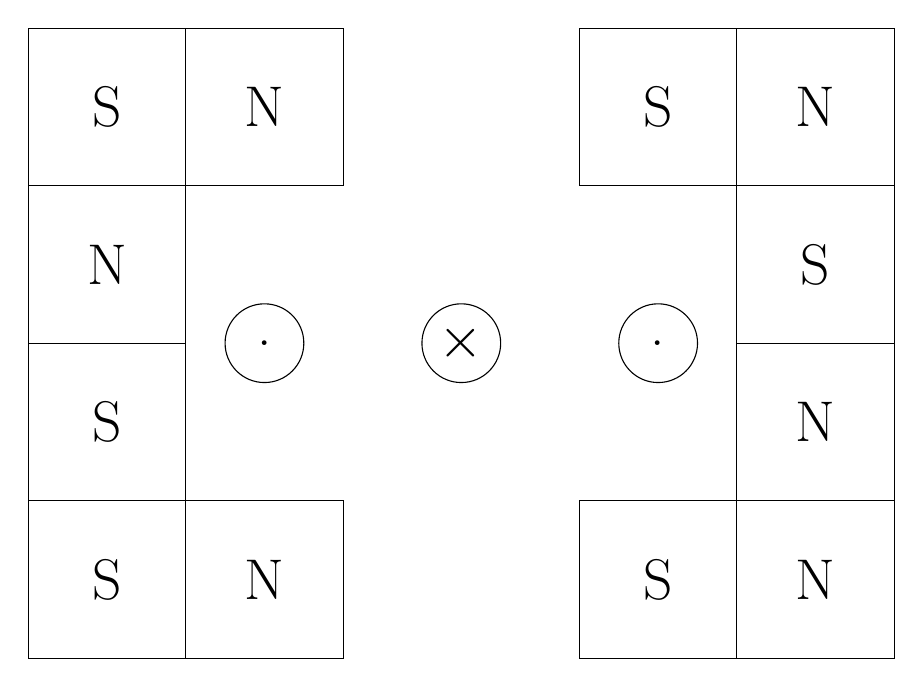
\begin{tikzpicture}
\draw (0,0)--(4,0)--(4,2)--(2,2)--(2,6)--(4,6)--(4,8)--(0,8)--(0,0);
\draw (2,2)--(0,2);
\draw (2,2)--(2,0);
\draw (2,4)--(0,4);
\draw (2,6)--(0,6);
\draw (2,6)--(2,8);
\draw (3,1) node {\huge N};
\draw (1,1) node {\huge S};
\draw (1,5) node {\huge N};
\draw (1,3) node {\huge S};
\draw (3,7) node {\huge N};
\draw (1,7) node {\huge S};

\draw (7,0)--(11,0)--(11,8)--(7,8)--(7,6)--(9,6)--(9,2)--(7,2)--(7,0);
\draw (9,2)--(9,0);
\draw (9,2)--(11,2);
\draw (9,4)--(11,4);
\draw (9,6)--(11,6);
\draw (9,6)--(9,8);

\draw (8,1) node {\huge S};
\draw (10,1) node {\huge N};
\draw (10,3) node {\huge N};
\draw (10,5) node {\huge S};
\draw (10,7) node {\huge N};
\draw (8,7) node {\huge S};

\draw (5.5,4) node {\huge $\times$} circle[radius=0.5] ;
\draw (3,4) node {\huge .} circle[radius=0.5] ;
\draw (8,4) node {\huge .} circle[radius=0.5] ;


\end{tikzpicture}
\end{center}
\end{document}